\documentclass[../main]{subfiles}
\begin{document}

\section{
  Brainfuck parsing and code generation
}
\label{lbl:bf-parsing-and-codegen}

Now that we introduced the various techniques to generate programs from
pointer trees generated by \gls{constexpr} functions, we will use them in the
context of compile time parsing and code generation for the Brainfuck language.
Therefore use data structures and code generation techniques introduced in
section \ref{lbl:ptr-tree-codegen}.

We chose Brainfuck as a first language for several reasons: the language
generates approximately one \gls{ast} node per character which makes the size
estimation of an \gls{ast} trivial, and the simplicity of the language allows us
to focus solely on code generation technicalities.

\subsection{
  Constexpr Brainfuck parser and AST
}

The Brainfuck \gls{ast} is defined in the header shown in appendix
\ref{app:bf-ast}. The header file also contains helper function definitions
to handle \gls{ast} nodes safely, such as \lstinline{visit} which will be used
in one of the code generation backends.

Here are the main data types:
\begin{itemize}
\item
\lstinline{node_interface_t}, which is a common base type for all \gls{ast} nodes.

\item
\lstinline{ast_token_t}, which represents a single \gls{ast} token.

\item
\lstinline{ast_block_t}, which represents an \gls{ast} block, which simply is a
\lstinline{std::vector} of \lstinline{std::unique_ptr<node_interface_t>}.

\item
\lstinline{ast_while_t}, which represents a while conditional block.
The instruction block itself is contained in an \lstinline{ast_block_t} value.

\end{itemize}

The implementation of the \gls{ast} are available in appendix \ref{app:bf-ast}
where you can observe that all the types are implemented as they would be
for a regular Brainfuck parser, except all their methods are \gls{constexpr}.

\clearpage%

\begin{lstlisting}[
  language=c++,
  caption=Definition of the \gls{ast} visitor function,
  label=lst:bf-ast-visit-def
]{}
template <typename F>
constexpr auto visit(F f, ast_node_ptr_t const &p) {
  switch (p->get_kind()) {
  case ast_token_v:
    return f(static_cast<ast_token_t const &>(*p));
  case ast_block_v:
    return f(static_cast<ast_block_t const &>(*p));
  case ast_while_v:
    return f(static_cast<ast_while_t const &>(*p));
  }
}
\end{lstlisting}

The \lstinline{visit} function implementation also looks like a regular \cpp
function as shown in listing \ref{lst:bf-ast-visit-def}.
It is a higher order function that allows recursive operations on the \gls{ast}
to be carried in a type-safe manner.
\\

The Brainfuck parser, again, looks like nothing special. For that reason I will
not get into the implementation details. The function definition is available
in appendix \ref{app:bf-parser}.

On the surface: the parser takes a pair of begin and end iterators as an input.
It parses Brainfuck tokens until it reaches the end iterator or a while end
token, and returns a pair containing an iterator pointing after the last parsed
token and the parsing result.

When a while begin token is reached, it calls itself recursively and resumes
parsing at the position of the iterator returned by the callee, which is right
after the while block.

The main parsing function implementation (including the function prototype)
is very compact: it fits in 40 lines of code with a max line width set to 84.
It is no different from a regular Brainfuck parsing function except for it being
\gls{constexpr}, and it can actually be used as a regular \cpp program.

These make it much easier to debug as it can be ran through a \cpp debugger like
GDB or LLDB, and also more maintainable as it does not require any
template metaprogramming experience to understand the implementation.
Additionally, \gls{constexpr} execution enforces checks on memory allocations and
deallocations as well as memory bound checking. Therefore testing functions
in \gls{constexpr} contexts can help finding memory safety issues.

Once the \gls{constexpr} parser is implemented, the next step consists in
figuring out how to transform its result, which contains dynamic memory,
into \cpp code.

As you may remember from section \ref{lbl:constexpr-programming},
there is no direct way to use values holding pointers to dynamic memory
directly as \glspl{nttp}.
Therefore it must be conveyed by other means or transformed into \glspl{litval}
to be used as template parameters for \cpp code generation.

I implemented several of these workarounds to compare them.
This will give us a clearer idea of their implementation difficulty,
and they will enable us to run compilation time benchmarks to compare their
compilation time performance.

\subsection{
  Pass-by-generator and Expression Template backends
}

The first backend implemented in the poacher project was the \gls{et} backend,
where the AST is transformed into a type-based \gls{ir}
as described in section \ref{lbl:pbg-et-technique}. It was later simplified to
remove the \gls{ir} transformation step, which gave the \gls{pbg} backend.

\begin{lstlisting}[
  language=c++,
  caption=\gls{et} backend \gls{ir},
  label=lst:bf-et-ir
]{}
template <typename... Nodes> struct et_block_t {
  constexpr et_block_t() {}
  constexpr et_block_t(Nodes const &...) {}
};

template <typename... Nodes> struct et_while_t {
  constexpr et_while_t() {}
  constexpr et_while_t(Nodes const &...) {}
};

template <token_t Token> struct et_token_t {};
\end{lstlisting}

The implementations of these two backends do not differ significantly from
the ones described in sections \ref{lbl:pbg-technique} and \ref{lbl:pbg-et-technique}:
the generators that evaluate each node are passed as template parameters,
only to work around the fact that pointers to \gls{constexpr} allocated memory
cannot be used in a \gls{nttp}.

Listing \ref{lst:bf-et-ir} shows the type-based \gls{ir} used for the \gls{et}
backend. \lstinline{et_block_t} and \lstinline{et_while_t} structures contain a
pack of arbitrary types that may be \lstinline{et_token_t} elements for single
tokens, or \lstinline{et_while_t} elements for nested while loops.

From there, the code generation occurs in the same way as it did in section
\ref{lbl:pbg-et-technique}: the \gls{et} is traversed recursively using
overloaded functions to generate the \cpp code that corresponds to every
while block, and down to every instruction in the \gls{et}.
The complete implementations of these backends are available in appendices
\ref{app:bf-et-backend} and \ref{app:bf-pbg-backend}.

\subsection{
  Serializing the \gls{ast} into a \gls{litval}
}

The last remaining backend to implement is the one that transforms
the \gls{ast} into a serialized, \gls{nttp} compatible \gls{ir}.
The case of Brainfuck introduces a notable difference compared to the simple
use case seen in section \ref{lbl:flat-technique}: while \gls{ast} nodes in Brainfuck
can have an arbitrary number of children nodes, as opposed to add nodes in
the simple use case I presented earlier. This introduces a few technical
differences with regard to serialization and code generation, which I will
cover in detail in this section.

\begin{lstlisting}[
  language=c++,
  caption=\gls{pbg} \gls{ir} type definitions,
  label=lst:flat-ir-typedef
]{}
/// Represents a single instruction token
struct flat_token_t {
  token_t token;
};

/// Block descriptor at the beginning of every block
/// of adjacent instructions.
struct flat_block_descriptor_t {
  size_t size;
};

/// Represents a while instruction, pointing to
/// another instruction block
struct flat_while_t {
  size_t block_begin;
};

/// Polymorphic representation of a node
using flat_node_t =
    std::variant<flat_token_t,
                 flat_block_descriptor_t,
                 flat_while_t>;

/// AST container type
using flat_ast_t = std::vector<flat_node_t>;

/// NTTP-compatible AST container type
template <size_t N>
using fixed_flat_ast_t = std::array<flat_node_t, N>;
\end{lstlisting}

Listing \ref{lst:flat-ir-typedef} shows the definition of the serialized
Brainfuck \gls{ir}. It is similar to the \gls{ir} in \ref{lbl:flat-technique},
except that it can represent ranges of instructions through
\lstinline{flat_block_descriptor_t}. This representation of node blocks
implies that nodes within the same block must be stored contiguously
after the serialization process.

To guarantee that nodes remain contiguous, the serialization process was split
in two parts: a first phase that generates a vector of blocks where references
are materialized by indexes to the blocks within that vector of vectors,
and a second phase that merges these blocks together into a single vector,
and replaces the block indexes by the beginning position of their subrange
in the result of the merging process.

\clearpage%

\begin{lstlisting}[
  language=c++,
  caption=\lstinline{block_gen_state_t} definition,
  label={lst:flat-block_gen_state_t}
]{}
struct block_gen_state_t {
  /// Flat AST blocks, result of block_gen
  std::vector<flat_ast_t> blocks;

  /// Keeping track of which block is being generated
  size_t block_pos = 0;

  /// Keeping track of the size of the AST
  size_t total_size = 0;
};
\end{lstlisting}

In listing \ref{lst:flat-block_gen_state_t} we begin by defining the structure
called \lstinline{block_gen_state_t} that contains the result of the first
serialization phase, and other useful values for the serialization process.

\begin{lstlisting}[
  language=c++,
  caption=Generic \lstinline{block_gen} implementation,
  label=lst:flat-block_gen-generic
]{}
/// Extracts an AST into a vector
/// of blocks of contiguous operations
constexpr void block_gen(ast_node_ptr_t const &,
                         block_gen_state_t &);

// Node-specific overloads...

constexpr void block_gen(ast_node_ptr_t const &p,
                         block_gen_state_t &s) {
  visit([&s](auto const &v) { block_gen(v, s); }, p);
}
\end{lstlisting}

Listing \ref{lst:flat-block_gen-generic} shows the implementation of the generic
version of \lstinline{block_gen}. It consists in a forward declaration
followed by node-specific implementations which call the generic version
recursively thanks to the  \lstinline{visit} function.
Specialized overloads of the \lstinline{block_gen} function follow the same
interface: they are invoked with a node and the state of the block generation
process as a mutable reference.

Listing \ref{lst:flat-block_gen-impl} shows the implementation of
\lstinline{block_gen} overloads for all types derived from
\lstinline{node_interface_t}.

The most important one is the overload for \lstinline{ast_block_t}.
It transfers each block in the \lstinline{blocks} vector
of the \lstinline{block_gen_state_t} structure by allocating them in the vector,
and calling \lstinline{block_gen} recursively for each node in the source block
to effectively transfer them into the destination block.

Once the vector of blocks is generated, the \lstinline{flatten} function
is responsible for transforming the contents of \lstinline{block_gen_state_t}
into such a representation.

\clearpage%

\begin{lstlisting}[
  language=c++,
  caption=Specialized \lstinline{block_gen} overloads,
  label={lst:flat-block_gen-impl}
]{}
/// block_gen for a single AST token.
constexpr void block_gen(ast_token_t const &tok,
                         block_gen_state_t &s) {
  s.blocks[s.block_pos].push_back(
      flat_token_t{tok.token});
}

/// block_gen for an AST block.
constexpr void block_gen(ast_block_t const &blo,
                         block_gen_state_t &s) {
  // Save & update block pos before adding a block
  size_t const previous_pos = s.block_pos;
  s.block_pos = s.blocks.size();
  s.blocks.emplace_back();

  // Preallocating
  s.blocks[s.block_pos].reserve(blo.content.size() + 1);
  s.total_size += blo.content.size() + 1;

  // Adding block descriptor as a prefix
  s.blocks[s.block_pos].push_back(
      flat_block_descriptor_t{blo.content.size()});

  // Flattening instructions
  for (ast_node_ptr_t const &node : blo.content) {
    block_gen(node, s);
  }

  // Restoring block pos after recursive block
  // processing
  s.block_pos = previous_pos;
}

/// block_gen for a while instruction.
constexpr void block_gen(ast_while_t const &whi,
                         block_gen_state_t &s) {
  s.blocks[s.block_pos].push_back(
      flat_while_t{s.blocks.size()});
  block_gen(whi.block, s);
}
\end{lstlisting}

Listing \ref{lst:flat-flatten-impl} shows the implementation of
\lstinline{flatten} which calls \lstinline{block_gen},
chains the blocks together, and translates block indexes to account for
the new layout.

The postfix serialization layout (ie. the fact that blocks are laid out
one after the other, and not one inside the other) ensures that
traversing the \gls{ast} remains trivial.

\clearpage%

\begin{lstlisting}[
  language=c++,
  caption=\lstinline{flatten} implementation,
  label={lst:flat-flatten-impl}
]{}
constexpr flat_ast_t
flatten(ast_node_ptr_t const &parser_input) {
  flat_ast_t serialized_ast;

  // Extracting as vector of blocks
  block_gen_state_t bg_result;
  block_gen(parser_input, bg_result);

  // Small optimization to avoid reallcations
  serialized_ast.reserve(bg_result.total_size);

  // block_map[i] gives the index of
  // bg_result.blocks[i] in the serialized
  // representation
  std::vector<size_t> block_map;
  block_map.reserve(bg_result.blocks.size());

  // Step 1: flattening
  for (flat_ast_t const &block : bg_result.blocks) {
    // Updating block_map
    block_map.push_back(serialized_ast.size());

    // Appending instructions
    std::ranges::copy(
        block, std::back_inserter(serialized_ast));
  }

  // Step 2: linking
  for (flat_node_t &node : serialized_ast) {
    if (std::holds_alternative<flat_while_t>(node)) {
      flat_while_t &w_ref =
          std::get<flat_while_t>(node);
      w_ref.block_begin =
          block_map[w_ref.block_begin];
    }
  }

  return serialized_ast;
}
\end{lstlisting}


From there, the only thing that needs to be done is to evaluate this
dynamic array into a static one to make it usable as an \gls{nttp}.
Listing \ref{lst:flat-parse-to-fixed-flat-ast-implementation} shows the
implementation of the final function that takes a string as a program
and transforms it into a \lstinline{fixed_flat_ast_t}.

So far, this is the only function that takes a template parameter as an input,
and thus where the distinction between \gls{constexpr} programming and \gls{tmp}
begins.

\clearpage%

\begin{lstlisting}[
  language=c++,
  caption=\lstinline{parse_to_fixed_flat_ast} implementation,
  label={lst:flat-parse-to-fixed-flat-ast-implementation}
]{}
/// Parses a BF program into a fixed_flat_ast_t value.
template <auto const &ProgramString>
constexpr auto parse_to_fixed_flat_ast() {
  // Getting AST vector size into a constexpr variable
  constexpr size_t AstArraySize =
      flatten(parser::parse_ast(ProgramString))
          .size();

  // Initializing static size array
  fixed_flat_ast_t<AstArraySize> arr;
  std::ranges::copy(
      flatten(parser::parse_ast(ProgramString)),
      arr.begin());

  return arr;
}
\end{lstlisting}

All the remaining work consists in implementing a function that takes the
serialized \gls{ast} as a template parameter and generates a program from it.

\begin{lstlisting}[
  language=c++,
  caption=\lstinline{program_state_t} definition,
  label=lst:program_state_t-def
]{}
struct program_state_t {
  constexpr program_state_t() : i(0) {
    for (auto &c : data) {
      c = 0;
    }
  }

  std::array<char, 30000> data;
  std::size_t i;
};
\end{lstlisting}

The functions generated by the codegen functions must take a reference to a
\lstinline{program_state_t} value to execute Brainfuck code.
The program state structure definition is shown in listing
\ref{lst:program_state_t-def}.

The implementation principle for the code generation functions is to visit
nodes recusively to compose and generate lambdas.
We will explore two ways to implement the \gls{ast} traversal:
one based on a monolithic implementation based on function overloading
to differentiate each type of node, and another one based on
\lstinline{if constexpr}.
\\


The \textbf{overloaded} version consists in a code generation entry point function
that selects instruction-specific code generation functions depending
on the type of token stored in the current instruction.

\clearpage%

\begin{lstlisting}[
  language=c++,
  caption=Overloaded \lstinline{codegen} entry point function,
  label=lst:ol-codegen-entrypoint
]{}
// Necessary forward declaration
template <auto const &Ast,
          size_t InstructionPos = 0>
constexpr auto codegen();

// Specialization implementations...

/// Generic code generation entrypoint
template <auto const &Ast, size_t InstructionPos>
constexpr auto codegen() {
  constexpr flat_node_t Instr =
      Ast[InstructionPos];

  // Calling specialized codegen versions
  // using function overloading
  return codegen<Ast, InstructionPos>(
      decltype(get<Instr.index()>(Instr)){});
}
\end{lstlisting}

Listing \ref{lst:ol-codegen-entrypoint} shows the implementation
of the entry point function whose only purpose is to unwrap the type
of the current element and use it to call the appropriate code generation
function depending on the instruction type.
The dispatch is done automatically through function overloading.

\begin{lstlisting}[
  language=c++,
  caption={
    \lstinline{codegen} specialization for \lstinline{flat_token_t} elements
  },
  label=lst:ol-codegen-token
]{}
template <auto const &Ast,
          size_t InstructionPos = 0>
constexpr auto codegen(flat_token_t) {
  // Extracting token value
  constexpr flat_token_t Token =
      get<flat_token_t>(Ast[InstructionPos]);

  // Returning code for a single Brainfuck
  // instruction

  // >
  if constexpr (Token.token ==
                pointer_increase_v) {
    return [](program_state_t &s) { ++s.i; };
  }
  // <
  else if constexpr (Token.token ==
                     pointer_decrease_v) {
    return [](program_state_t &s) { --s.i; };
  }

  // More instructions...
}
\end{lstlisting}

In listing \ref{lst:ol-codegen-token} we can see the implementation of a
code generation function for simple instructions, \ie any instruction
represented by a token that isn't a while block delimiter.
The dispatch over the tokens is done using \lstinline{if constexpr},
but it could have been done using a variable template with
template specializations for each case.

Note that the token passed as a regular parameter is only used for the overload
selection. The token value used to evaluate conditions in the
\lstinline{if constexpr} statements is sourced from the \gls{ast} passed as a
\gls{nttp}, therefore it is still \gls{constexpr}.

\begin{lstlisting}[
  language=c++,
  caption={
    \lstinline{codegen} specialization
    for \lstinline{flat_block_descriptor_t} elements
  },
  label=lst:ol-codegen-block
]{}
/// Code generation implementation
/// for a code block
template <auto const &Ast,
          size_t InstructionPos = 0>
constexpr auto codegen(flat_block_descriptor_t) {
  return [](program_state_t &s) {
    // Generating an index sequence type
    // with a size equal to the code block size.
    // It will be passed to the template lambda
    // to expand its indexes.
    auto index_sequence =
        std::make_index_sequence<
            get<flat_block_descriptor_t>(
                Ast[InstructionPos])
                .size>{};

    // Static unrolling on the block's
    // instructions, made possible by the
    // contiguity of its elements
    [&]<size_t... Indexes>(
        std::index_sequence<Indexes...>) {
      // Expansion on the index to generate code
      // for each node and invoke it with the
      // program state
      (..., codegen<Ast, 1 + InstructionPos +
                             Indexes>()(s));
    }(index_sequence);
  };
}
\end{lstlisting}

The trickiest part of code generation is generating code blocks, as shown in
listing \ref{lst:ol-codegen-block}. Doing so requires the use of a compile time
unrolling technique based on \cpp parameter packs.
Iteration over the elements must be done that way to keep the index
\gls{constexpr} and use it as a \gls{nttp} to generate code.

The result of this metafunction is an anonymous function that evaluates all the
Brainfuck code within a block. At this point the only function that remains
is the \lstinline{flat_while_t} overload.

\begin{lstlisting}[
  language=c++,
  caption={
    \lstinline{codegen} specialization
    for \lstinline{flat_while_t} elements
  },
  label=lst:ol-codegen-while
]{}
/// Code generation implementation for a while block
template <auto const &Ast, size_t InstructionPos = 0>
constexpr auto codegen(flat_while_t) {
  return [](program_state_t &s) {
    while (s.data[s.i]) {
      codegen<Ast, get<flat_while_t>(Ast[InstructionPos])
                       .block_begin>()(s);
    }
  };
}
\end{lstlisting}

The \lstinline{codegen} implementation for a while block
\ref{lst:ol-codegen-while} is trivial: it returns a function that runs a while
loop as defined by the Brainfuck language specification, and the body itself is
the code generation result for the block element it points to.
This implementation is a good way to illustrate code generation from a
\gls{nttp} for a serialized \gls{ast}.

\begin{lstlisting}[
  language=c++,
  caption={\lstinline{if constexpr} based \lstinline{codegen} implementation},
  label=lst:icx-codegen
]{}
template <auto const &Ast,
          size_t InstructionPos = 0>
constexpr auto codegen() {
  constexpr flat_node_t Instr =
      Ast[InstructionPos];

  if constexpr (holds_alternative<flat_token_t>(
                    Instr)) {
    constexpr flat_token_t Token =
        get<flat_token_t>(Instr);
    // Single token code generation...
  }

  else if constexpr (holds_alternative<
                         flat_block_descriptor_t>(
                         Instr)) {
    constexpr flat_block_descriptor_t
        BlockDescriptor =
            get<flat_block_descriptor_t>(Instr);
    // Block code generation...
  }

  else if constexpr (holds_alternative<
                         flat_while_t>(Instr)) {
    constexpr flat_while_t While =
        get<flat_while_t>(Instr);
    // While loop code generation...
  }
}
\end{lstlisting}

A \textbf{monolithic} implementation of \lstinline{codegen} can be implemented by
replacing overloading with \lstinline{if constexpr} and
\lstinline{std::holds_alternative}.

Listing \ref{lst:icx-codegen} shows the \lstinline{if constexpr} based
code generation implementation. Note that bits of code were cut to make
the listing shorter, but they are the same as the overloaded \lstinline{codegen}
overload function bodies. This \lstinline{codegen} implementation remains
functionally identical to the previous one.

\subsubsection{
  Variable-sized benchmarks
}
\label{lbl:compile-time-eval}

We first begin by running two variable-sized benchmarks, consisting in
measuring compiler execution time as the \gls{ast} widens, and as the \gls{ast}
deepens.
\\

The first variable-sized benchmark consists in generating a valid BF \gls{ast} by
concatenating strings to generate a succession of BF while loops in a
\gls{constexpr} string. This benchmark was instantiated with sizes going from 1 to
10 with a step of 1, with 10 timing iterations for each size.
The second benchmark generates a string with
nested loops, making the \gls{ast} deeper as the benchmark size increases
instead of making it wider as in the previous case. Both benchmarks generate
programs of the same size.

\begin{figure}[h]
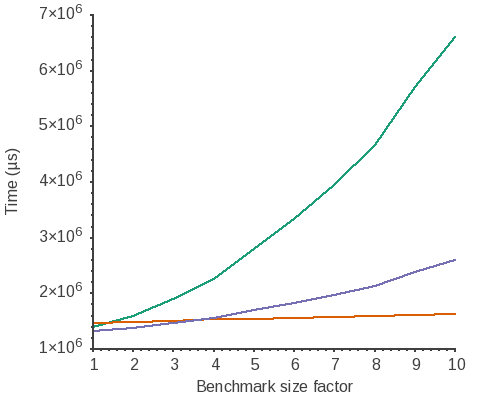
\includegraphics[scale=0.5]{images/bf-consecutive_loops.png}
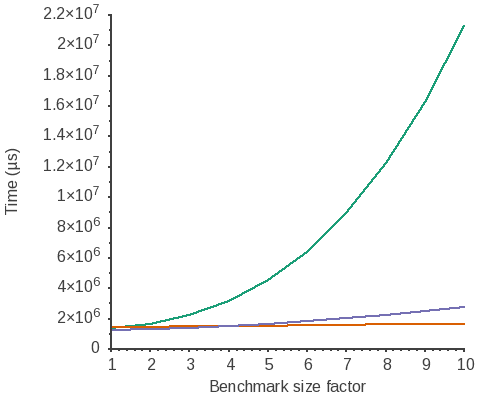
\includegraphics[scale=0.5]{images/bf-imbricated_loops.png}
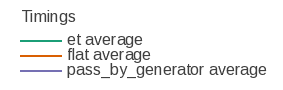
\includegraphics[scale=0.5]{images/bf-graph-legend.png}
\caption{
  Compiler execution time measurements for consecutive loops (left)
  and nested loops (right)
}\label{fig:bf-bench}
\end{figure}

Figure \ref{fig:bf-bench}
highlights considerably higher compiler execution times for the expression
template based backend, high enough to suggest that the use of expression
templates induces an overhead higher than parsing and generating Brainfuck
programs using the \gls{pbg} backend. However the \gls{pbg}
backend still has a compile time overhead much higher than the flat backend,
which shows near constant compiler execution times on these small scale
benchmarks.

Finally, \gls{ast} deepening has a much higher impact on compile times than
\gls{ast} widening with the expression template backends,
whereas the other backends seem to scale similarly as the \gls{ast}
grows wider or deeper.

\subsubsection{
  Large Brainfuck programs
}
\label{lbl:bf-large-program-benches}

The following benchmarks consist in measuring compiler execution times for
compiling Brainfuck code examples. These example programs are also used to
validate the metacompiler's backend implementations by compiling them and
verifying their output.

\begin{itemize}
\item A Hello World program (106 tokens).
\item The same Hello World program, ran twice (212 tokens).
\item A Mandelbrot set fractal viewer (11672 tokens).
\end{itemize}

\begin{figure}[h]
\begin{tabular}{|c|c|c|c|}
\hline
Backend           & Hello World & Hello World x2  & Mandelbrot \\
\hline
Flat (Monolithic) & 0.63        & 0.80            & 18.16 \\
Flat (Overloaded) & 0.66        & 0.90            & 28.51 \\
\gls{pbg}         & 3.55        & 12.73           & Failure (timeout) \\
\gls{et}          & 19.18       & 74.51           & Failure (timeout) \\
\hline
\end{tabular}
\caption{Brainfuck compile time measurements in seconds}
\label{fig:bf-compile-times}
\end{figure}

The measurements in figure \ref{fig:bf-compile-times} help us better assess
how various metacompiling techniques behave at scale.
The Hello World program is meant to represent a simple embedded expression,
while the Mandelbrot visualization is a much larger program meant to represent
an upper bound of what a \gls{dsel} would be reasonably used for as it is more
than 200 lines of code.

However, proposals such as \lstinline{std::embed} \cite{stdembed}
could dramatically increase the size of embedded programs as whole source files
could be used directly as embedded expressions or programs in \cpp.

\subsubsection{
  Conclusion
}

Here is what can be said about each backend:

\begin{itemize}

\item
\textbf{Flat backends}:
they are not the easiest to implement due to the additional \gls{ir}
and serialization step that need to be implemented.

However, they present clear benefits when it comes to compilation times.
So far they are the only ones that can be used at scale.
The Mandelbrot example is supposed to illustrate an extreme case where
\glspl{dsel} are used to integrate large programs (approximately 11'000
\gls{ast} nodes), and yet both "flat" implementations manage to keep compilation
times well under a minute.

\item
\textbf{\gls{pbg} backend}:
The \gls{pbg} backend has the shortest implementation.
However, it might not be the least difficult to implement.

The code examples do not reflect the time spent debugging \gls{constexpr}
allocated memory errors. While the \gls{pbg} may be a decent route for
rapid prototyping to compile simple embedded expressions or programs,
its poor performance scaling might be an issue.

Judging from the implementation, the initial hypothesis was that its
compilation time complexity as a function of program size would be quadratic
and was confirmed by a compilation time analysis.
This hypothesis was confirmed by compilation time benchmarks on small
and large scale programs.

\item
\textbf{\gls{et} backend}:
This backend was originally meant to be a demonstrator for the interoperability
of \gls{constexpr} memory and \glspl{et}. It shows no particular advantage
compared to the two other backends: it is slower than the \gls{pbg} backend while
requiring additional effort to implement the \gls{et}
\gls{ir}.

\end{itemize}

As a broad conclusion for compile time Brainfuck code generation,
it can be said that using \gls{nttp}-based techniques to generate code
is preferable in order to avoid compilation times to increase dramatically.

\end{document}
